\chapter{Median Finding in Linear Time}

\begin{algoprob}
	\problemtitle{\textsc{Median-Find}($S$)}
	\probleminput{Set $S$ of $n$ distinct integers}
	\problemquestion{Find the $\lt\lfloor\frac{n}{2}\rt\rfloor^{th}$ smallest integer in $S$}
\end{algoprob}

\section{Naive Algorithm}
The naive algorithm for this will be to sort the array in $O(n\log n)$ time then return the  $\lt\lfloor\frac{n}{2}\rt\rfloor^{th}$ element. This will take $O(n\log n)$ time. But in the next section we will show a linear time algorithm.

\section{Linear Time Algorithm}
In this section we will show an algorithm to find the median of a given set of distinct integers in $O(n)$ time complexity. We will follow \cite[Section 9.3]{CormenThomasLeisersonCharlesRivestRonaldSteinClifford_BOOK}. Consider the following two problems:

\begin{algoprob}
	\problemtitle{\textsc{Rank-Find} ($S,k$)}
	\probleminput{Set $S$ of $n$ distinct integers and an integer $k\leq n$}
	\problemquestion{Find the $k^{th}$ smallest integer in $S$}
\end{algoprob}
\begin{algoprob}
	\problemtitle{\textsc{Approximate-Split}($S$)}
	\probleminput{Set $S$ of $n$ distinct integers}
	\problemquestion{Given $S$, return an integer $z\in S$ such that $z$ where $rank(z)\in \lt[\frac{n}{4},\frac{3n}{4}\rt]$}
\end{algoprob}

%Certainly \prb{Rank-Find}$(S,k)$ is harder than $\prb{Approximate-Split}$. 
\subsection{Solve \prb{Rank-Find} using \prb{Approximate-Split}}
%Here suppose we can solve $\prb{Approximate-Split}$ easily. Now we want to solve $\prb{Rank-Find}$ using $\prb{Approximate-Split}$.
\begin{algorithm}
	\DontPrintSemicolon
	\KwIn{Set $S$ of $n$ distinct integer and $k\in[n]$}
	\KwOut{$k^{th}$ smallest integer in $S$}
	\Begin{
%$n\longleftarrow |S|$\;
\If{$|S|\leq 100$}{Sort $S$, \Return{$k^{th}$ smallest element in $S$}}	
$z\longleftarrow \prb{Approximate-Split}(S)$\hspace{1cm}
($z$ is the $r^{th}$ smallest element for some $r\in \lt[\frac{n}{4},\frac{3n}{4}\rt]$)\;
$S_L\longleftarrow \{x\in S\mid x\leq z\}$, $S_R\longleftarrow \{x\in S\mid x>z\}$\;
\If{$k\leq |S_L|$}{\Return{\prb{Rank-Find}$(S_L,k)$}}
\Return{\prb{Rank-Find}$(S_R,k-|S_L|)$}
}
\caption{\prb{Rank-Find}(S,k)}
\end{algorithm}
\parinn

Certainly if we can solve $\prb{Rank-Find}(S,k)$ for all $k\in[n]$ we can also solve $\prb{Median-Find}$. We will try to use both the problems and recurse to solve \prb{Rank-Find} in linear time. 

In the above algorithm $rank(z)\in \lt[\frac{n}{4},\frac{3n}{4}\rt]$. So $\frac{n}4\leq |S_L|,|S_R|\leq \frac{3n}4$. For now suppose $\prb{Rank-Find}(S,k)$ takes $T_{RF}(n)$ time and $\prb{Approximate-Split}(S)$ takes $T_{AS}(n)$ time. Then the time taken by the algorithm is  $$T_{RF}(n)\leq O(n)+T_{AS}(n)+T_{RF}\lt(\frac{3n}4\rt)$$
\subsection{Solve \prb{Approximate-Split} using \prb{Rank-FInd}}
We first divide $S$ into groups of $5$ elements. So take $t=\lt\lceil\frac{n}5\rt\rceil$. Now we sort each group. Since each group have constant size this can be done in $O(n)$ time. So now consider the scenario:
\begin{figure}[h]
	\centering
	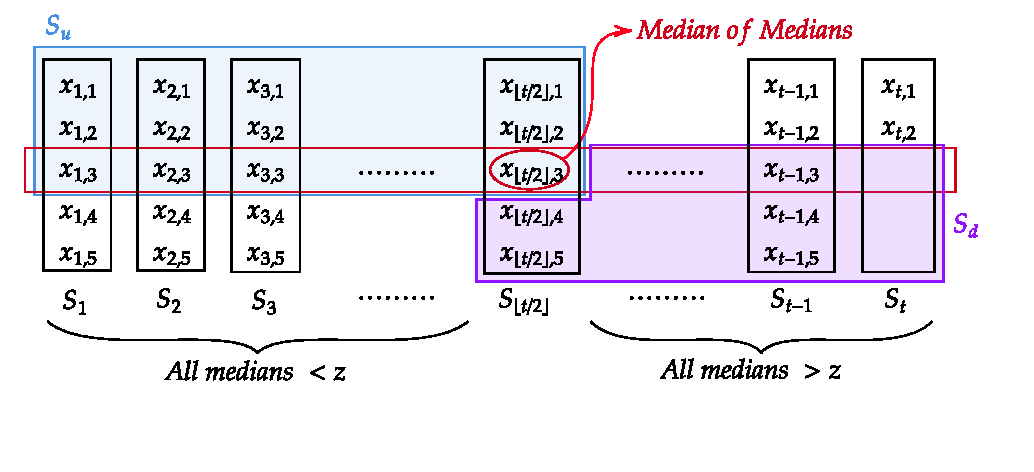
\includegraphics{images/approx-split-using-rankfind}
\end{figure}